\section{Cockcroft Walton}\label{ch:cock}
The Cockcroft-Walton Multiplier (CWM) utilises passive components to multiply a fluctuating voltage input.
The input voltage does not need to be a pure AC wave,
but also works with any DC shift,
as only the peak to peak amplitude is important for its function.\cite{Cockcroft1932}\\
A schematic of the CWM can be seen in Figure \ref{fig:CWM}.\\

\begin{figure}[H]
   \centering
   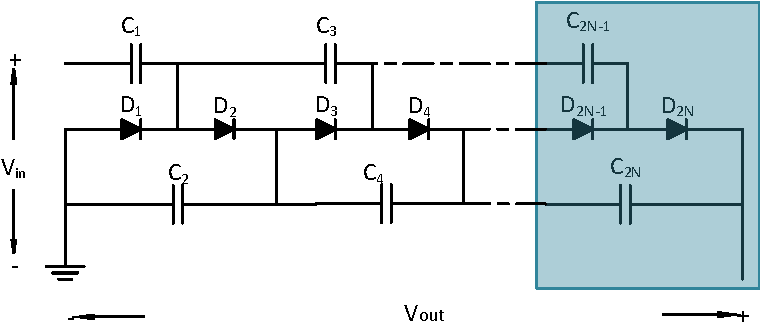
\includegraphics[width=0.8\textwidth]{figures/xCockroftWalton/CockroftWalton.pdf}
    \caption{Schematic of the Cockcroft-Walton Multiplier}
	\label{fig:CWM}
\end{figure}

%\subsection{Additions from Conventional BC}
The figure shows a two stage CWM,
with a third stage added (inside blue box).
Since all stages are equal and just appended to the previous,
more stages can be added at the dotted lines.

As mentioned before,
the CWM works on alternating input.
The Diodes in the middle row alternate between positive and reverse bias with each half wave.
Figure \ref{fig:CockBothWave} shows the circuit equivalents after removing the diodes in reverse bias for each half wave.
Subfigure \ref{sfig:1neg} shows the equivalent circuit with all capacitors discharged.
The following subfigures show the development of the circuit,
if the capacitors are to charge fully during one half wave.

%\subsection{Analysis of Individual Stage}
\begin{figure}[H]%
    \centering
    \subfloat[Negative half Wave\label{sfig:1neg}]{
    	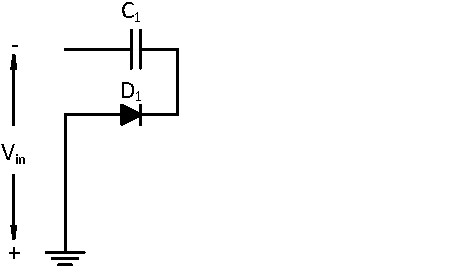
\includegraphics[width=0.45\textwidth]{figures/xCockroftWalton/1neg.pdf}
    }%
    \qquad
    \subfloat[Positive half Wave\label{sfig:2pos}]{
    	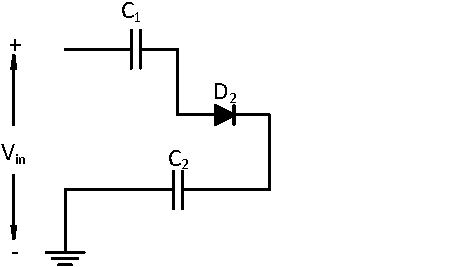
\includegraphics[width=0.45\textwidth]{figures/xCockroftWalton/2pos.pdf}
    }\\%  
    \subfloat[Negative half Wave\label{sfig:3neg}]{
    	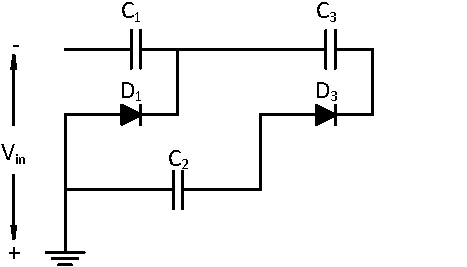
\includegraphics[width=0.45\textwidth]{figures/xCockroftWalton/3neg.pdf}
    }%
    \qquad
    \subfloat[Positive half Wave\label{sfig:4pos}]{
    	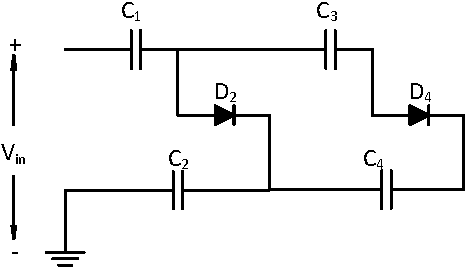
\includegraphics[width=0.45\textwidth]{figures/xCockroftWalton/4pos.pdf}
    }%  
    \caption{CWM Circuit Equivalents for Alternating $V_{in}$}%
    \label{fig:CockBothWave}% 
\end{figure}

When the upper terminal is negative with respect to ground,
the top capacitors (uneven numbers) are charged (Subfigures \ref{sfig:1neg} \& \ref{sfig:3neg}).
When the upper terminal is positive with respect to ground,
the bottom capacitors are charged (Subfigures \ref{sfig:2pos} \& \ref{sfig:4pos}).

This behaviour is possible through the placement of the diodes.
Every diode $D_n$ where $n > 1$ is forward biased under the condition shown in Equation \ref{eq:DiodeOnCW}.

\begin{equation}
	V_{C_{n-1}}-V_D \geq V_{C_n}
	\label{eq:DiodeOnCW}
\end{equation}

$D_1$ is always forward biased when the input voltage is on the negative half wave,
as it doesn't depend on a previous capacitor.
Therefore $C_1$ is charged directly by the input voltage.

As Equation \ref{eq:DiodeOnCW} states the forward bias condition of the diodes,
and holds until both capacitors are equally charged,
it can be expected that every capacitor $C_n$ will eventually acquire the same potential as $C_{n-1}$.
We proved this through simulation,
and Figure \ref{fig:capsV} shows the results.


\begin{figure}[H]
   \centering
   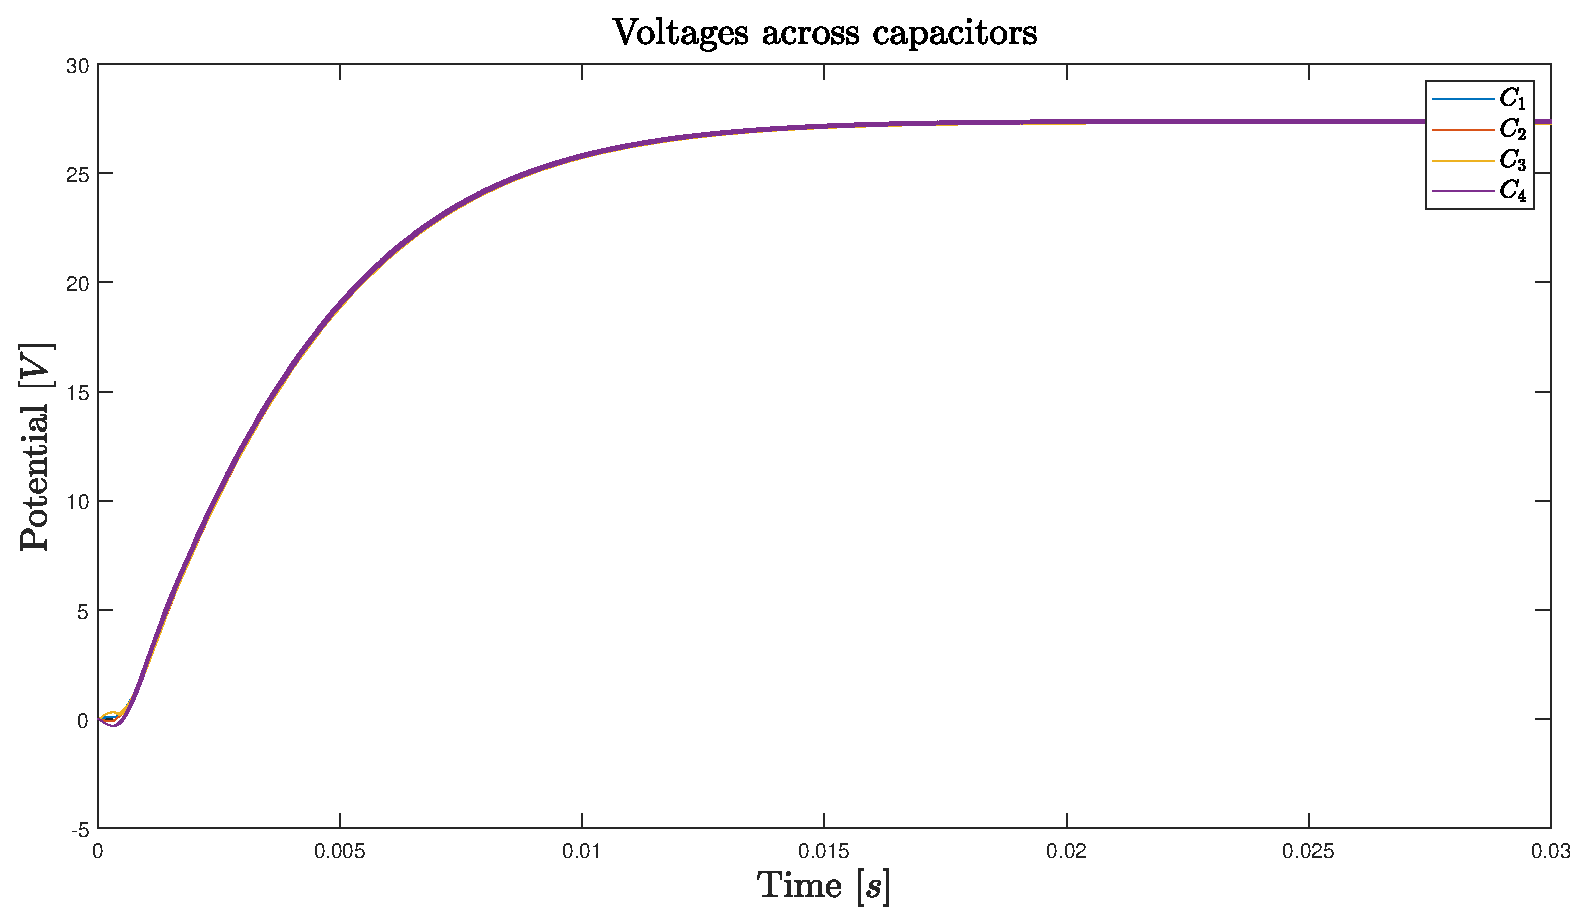
\includegraphics[width=0.8\textwidth]{figures/xCockroftWalton/capsV.eps}
    \caption{Voltages across Capacitors of a 2 Stage CWM}
	\label{fig:capsV}
\end{figure}
